%----------------------------------------------------------------------------------------
%	CONFIGURATIONS
%----------------------------------------------------------------------------------------

\documentclass[12pt,a4paper,oneside]{article}

\usepackage[utf8]{inputenc}
\usepackage{graphicx}
\usepackage{natbib}
\usepackage{amsmath}
\usepackage{caption}
\usepackage{subcaption}
\graphicspath{ {images/} }
\usepackage[a4paper,left=2cm,right=2cm,top=2.5cm,bottom=2.5cm]{geometry}
\setcounter{section}{-1}

%----------------------------------------------------------------------------------------
%	INFORMATION
%----------------------------------------------------------------------------------------

\title{Tópicos Avançados em Algoritmos (TAA) - Practical Assignment 1}

\author{João Rebelo Pires\footnote{João Rebelo Pires - 201200384} and José Miguel Oliveira\footnote{José Miguel Oliveira - 201304192}}

\date{DCC - FCUP, April 2017}

\begin{document}

\maketitle

%----------------------------------------------------------------------------------------
%	SECTION 0
%----------------------------------------------------------------------------------------

\section{How To}\label{sec:for_dummies}

In this section, we simply want to explain how to compile and execute our implementation.

\subsection{Input Description}\label{subsec:input_descrip}

The first line of input contains a single integer, an option. If this option is $0$, we are looking for the horizontal partition. Alternatively, the option may be $1$, indicating that we are looking for the grid partition.

The second line of input is an integer, $n\_vertices$, describing the number of vertices the orthogonal polygon has. Then $n\_vertices$ lines follow, the coordinates of the vertices of the polygon, given in counterclockwise order. The coordinates are integer.

The next line of input is an integer, $n\_holes$, describing the number of holes the polygon has. The following lines describe each hole, ina  similar way as the polygon is described.

\subsection{Output Description}\label{subsec:output_descrip}

The output is well represented. It consists on three groups of information.

\begin{enumerate}
	\item The description of each vertex of the DCEL;
	\item The description of each face of the DCEL;
	\item The description of each half edge of the DCEL.
\end{enumerate}

The information each element of the DCEL provides is discussed in section . %TODO \ref para a sec com isto

\subsection{Compilation}\label{subsec:compile}

The following command line compiles the code:

\textit{In MacOS X:}

\texttt{clang++ -Wall main.cpp code/dcelutil.cpp}\\

\textit{In Linux:}

\texttt{c++ -Wall main.cpp code/dcelutil.cpp}

\subsection{Execution}

The compiler generates an executable named \textbf{a.out}. To execute it, simply execute the following command line:

\texttt{./a.out}.\\

If you have an input file \textbf{test.in}, you should execute the following command line instead:

\texttt{./a.out < test.in}.

%----------------------------------------------------------------------------------------
%	SECTION 1
%----------------------------------------------------------------------------------------
\section{Introduction}
For this assignment we had the task of partitioning any orthogonal polygon with or without holes, then compute the visibility and finally study experimentally the minimum guard problem. 

We managed to complete the first of three parts by doing the horizontal and grid partition of the polygon.
We used a sweeping algorithm to accomplish the horizontal and vertical partitions. 
When doing the vertical partition we would rotate the polygon 90 degrees CCW and execute the same sweeping algorithm as for the horizontal partition.

%----------------------------------------------------------------------------------------
%	SECTION 2
%----------------------------------------------------------------------------------------
\section{DCEL Structure}
To represent the polygon with and without the partitions we are using a doubly connected edge list (DCEL).\\
This structure allows us to easily build and traverse the polygon, as it is built using the half edges of the polygon and each half edge has the following attributes:

\begin{enumerate}  
\item \textbf{Next}: The half edge that comes after the one we are analysing
\item \textbf{Incident}: The face in which that half edge is contained
\item \textbf{Twin}: The reverse half edge to the one we are analysing, used to navigate through the polygon in reverse
\item \textbf{Prev}: The half edge that comes before the one we are analysing
\item \textbf{Origin}: The vertex in which this half edge originates
\end{enumerate}

\begin{figure}[h!]
  \centering 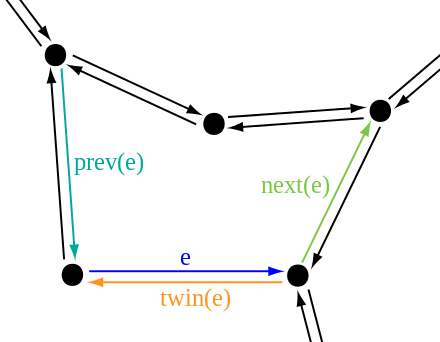
\includegraphics[scale=0.5]{dcel.png}
  \caption{DCEL}
  \label{fig:Dcel}
\end{figure}

% https://upload.wikimedia.org/wikipedia/commons/thumb/0/07/Dcel-halfedge-connectivity.svg/440px-Dcel-halfedge-connectivity.svg.png

Using these attributes we can easily print out the polygon and its partitions using the next attributes to navigate through each different face.

\pagebreak

%----------------------------------------------------------------------------------------
%	SECTION 3
%----------------------------------------------------------------------------------------
\section{Horizontal Partition}
To accomplish the horizontal partition, we used a sweeping algorithm.\\ 
A line would cross the polygon from the bottom up, find the intersections between these events (horizontal edges) and the walls of the polygon on both sides and then extend those events, splitting the polygon.
Intersections could occur between an inside vertex and a vertical polygon wall or between two inside vertexes.\\
Let's look at an example:

\begin{figure}[h!]
  \centering 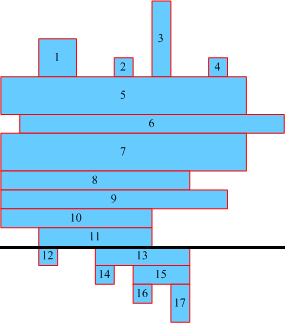
\includegraphics[scale=0.5]{horPartition.png}
  \caption{Horizontal Partition}
  \label{fig:Horizontal Partition}
\end{figure}

% http://www.yzuda.org/download/_CornerStitchingStrips/complex-02.png

The figure above, shows us how the horizontal partition of an orthogonal polygon. \\
The black horizontal line is the sweep line, that goes from event to event looking for possible edge extensions. Each event is a horizontal half edge. \\
We can see the different types of intersections that occur, which we mentioned previously. The intersection between two inside vertexes, as we can see at the bottom of rectangle 6, and the intersection between an inside vertex and the vertical polygon wall that can be seen at the top of the rectangle numbered 9.


%----------------------------------------------------------------------------------------
%	SECTION 4
%----------------------------------------------------------------------------------------
\section{Grid Partition}
For the grid partition we need both the horizontal and vertical partitions in place.\\
For the vertical partition we used a very similar idea to the horizontal one, with some slight differences.\\
We would "rotate" the polygon 90 degrees, and execute the horizontal partition. This would work because when the polygon is rotated, the vertical edges become horizontal and vice-versa, so if we were to execute the algorithm for the horizontal partition on the rotated polygon, and then rotate it back to the original position, the partition would become vertical.

\begin{figure}[h!]
  \centering 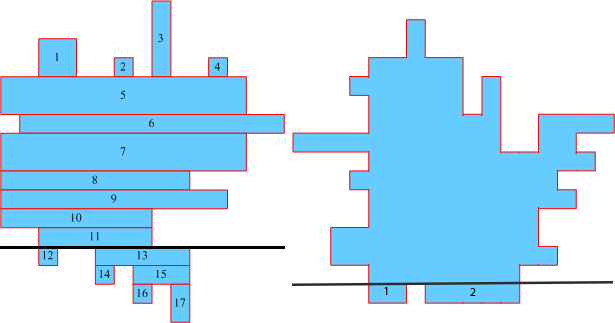
\includegraphics[scale=0.5]{rotatedPoly.png}
  \caption{Polygon Rotation}
  \label{fig:Dcel}
\end{figure}

\begin{figure}[h!]
  \centering 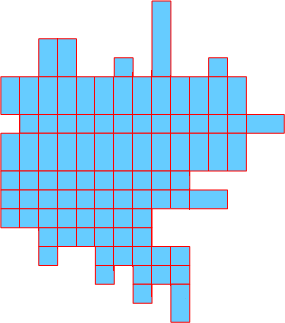
\includegraphics[scale=0.5]{gridPartition.png}
  \caption{Grid partition}
  \label{fig:Dcel}
\end{figure}

All that is left now to complete our grid partition, is to join both the horizontal and vertical partitions. We do that by finding the points of interest in the vertical partition. These points will be the intersections of both partitions.

\end{document}
